Классическая теория тестирования предполагает, что ответ на вопрос c вариантами ответа может быть представлена в виде
случайной бернулевской величины $\xi_i$ \cite{traub1997classical}. Итоговый результат прохождения тестирования представлен
в виде вектора $\mathbf{\xi} =(\xi_1,\dots,\xi_n)$. Теория предполагает вопросы независимыми и имеющими равную сложность, поэтому
знания учащегося представляет как сумму координат $\mathbf{\xi}$:
\begin{equation}
    s \sim \mathrm{N}(\theta,\sigma^2), 
\end{equation}
где $s$ задает экзаменационный результат обучаемого, параметр $\theta$ --- истинный уровень знания, 
$\sigma^2$ --- задает волатильность измерений. Параметр волатильности  считается равным для всех учащихся и подбирается
путем максимизации правдоподобия на экспериментальной выборке. Существенным недостатком такой теории является предположение 
о равной сложности задач для учащегося в контрольной работе. Контрольно-методические материалы, составленные по такой системе,
как правило, имеют бинарные ответы и проверяют лишь базовые предметные знания \cite{van1994likert}.  

\begin{figure}[h]
    \centering
    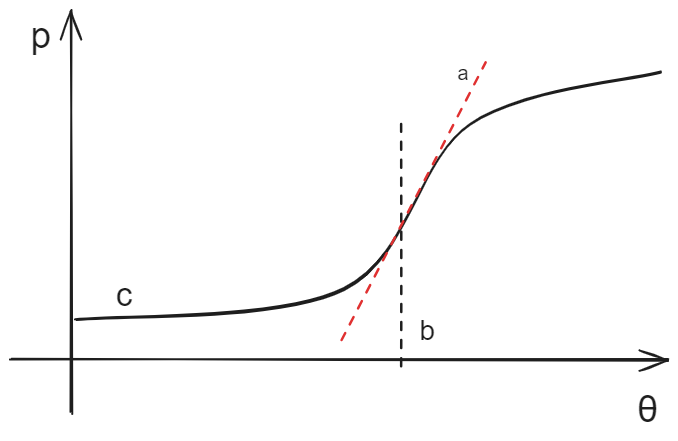
\includegraphics[width=0.5\textwidth]{assets/pedagogic/social/irt.excalidraw.png}
    \caption{Отклик учащегося на образовательный материал в теории IRT задается смещенной логистичеcкой функцией}
    \label{irt_function}
\end{figure}

Для работы с упорядоченным по сложности заданиями  институтом Educational Testing Service 
была создана теория отклика на материал (от \textit{англ.} Item Response Theory)\cite{lord2012applications}. 
Наиболее известным результатом теории является 3-х параметрическая логистическая модель \ref{irt_function}, учитывающая сложность задачи,
вероятность угадать правильный ответ и волатильность оценки \cite{lord1956measurement}:
\begin{equation}
    p_i(\theta) = c_i + \frac{1-c_i}{1+e^{-a_i(\theta-b_i)}},
\end{equation}
где $\theta$ --- текущий уровень навыков, $b_i$ --- сложность задания, $a_i$ --- характерный масштаб, $c$ --- вероятность угадать решение.
Выбор коэффициентов выполняется на экспериментальных данных путем оптимизации с помощью EM-алгоритма \cite{bock1981marginal}. 
Таким образом, каждая задача приобретает скалярный уровень сложности, используемый методистами для составления сбалансированных по сложности
контрольно-методических работ. 

Теория отклика используется при составлении контрольно-методических систем, значительно влияющих на 
профессиональные возможности экзаменуемого и репутацию образовательных систем,
\begin{itemize}
    \item международных экзаменов по математике GMAT, английскому языку: ILETS и TOEFL;
    \item программ оценки образовательных достижений PIZA и TIMSS;
    \item поступлении в американские колледжи SAT.  
\end{itemize}
Также теория отклика активно применяется  в современном персональном образовании c использованием 
информационно-коммуникационных систем (от \textit{англ.} Information and Communication System)\cite{abbott2003ict}
\cite{manouselis2011recommender}. Образовательные платформы по обучению языку Revita \cite{katinskaia2018revita}, математике
MathGarden \cite{straatemeier2014math} и программированию Stepik используют функцию отклика для адаптивного обучения,
подбирая сложность заданий исходя из текущих знаний учащегося. Такой подход, на текущий момент, формирует 
новое научное направление теории цифрового образования (от \textit{англ.} technology enhanced learning), объединяющей
рекомендательные и психометрические подходы для эффективного обучения \cite{manouselis2011recommender}.
\begin{figure}[h]
    \centering
    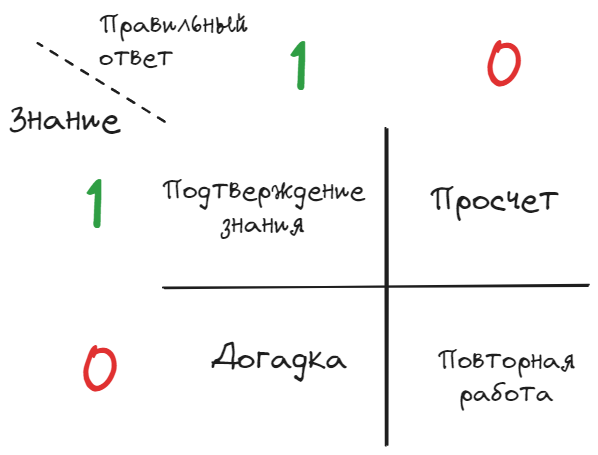
\includegraphics[width=0.5\textwidth]{assets/pedagogic/social/bkt.excalidraw.png}
    \caption{Эволюция представлений о знаниях учащегося}
    \label{bkt}
\end{figure}
Базовой моделью адаптивного алгоритма оценки знаний является байесов пересчет \cite{corbett1994knowledge}.
Модель учитывает вероятность ошибки и вероятность ошибиться при наличии знания \ref{bkt}: 
\begin{itemize}
    \item $P(L_0)$ --- начальные знания в предмете;
    \item $P(S) = P(x=0| L_t = 1)$ --- вероятность просчета при наличи знаний;
    \item  $P(G) = P(x=1| L_t = 1)$ --- вероятность угадать при отсутствии знаний.
\end{itemize}
Обновление представлений выполняется с учетом ответа согласно:
\begin{equation}
    \begin{aligned}
        &P(L_t| obs_t=1) = \frac{P(L_t)(1-P(S))}{P(L_t)(1-P(S)) + (1-P(L_t))P(G)} \\
        &P(L_t| obs_t=0) = \frac{P(L_t)P(S)}{P(L_t) P(S) + (1-P(L_t))(1-P(G))}.
    \end{aligned}
\end{equation}
Отметим, что полученный вывод предполагает, что:
\begin{itemize}
    \item вероятность забыть знание равна нулю $ P(L_{t+1}=0|L_t=1)=0$;
    \item вероятность наличия знаний обновляется по правилу $P(L_{t+1}) = P(L_t|obs_t) + \left(1 - P(L_t | obs_t)\right) P(T)$.
\end{itemize}
\begin{figure}[h]
    \centering
    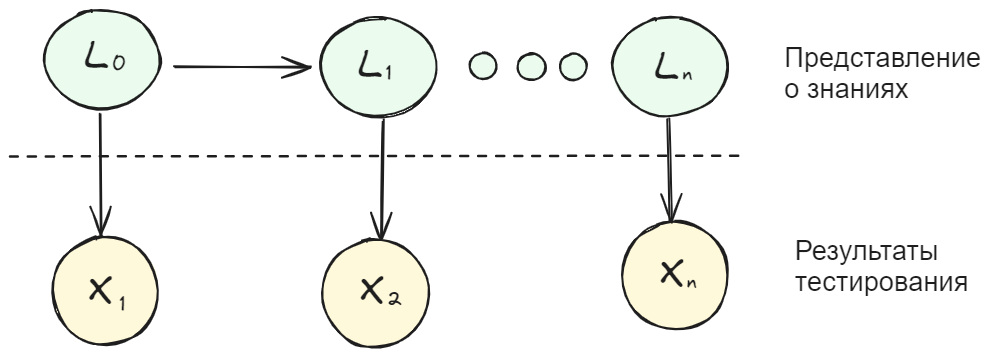
\includegraphics[width=0.7\textwidth]{assets/pedagogic/social/bkt_automata.excalidraw.png}
    \caption{Матрица исходов модели Байесовской оценки на шаге t}
    \label{bkt_automata}
\end{figure}
Таким, образом тест можно представить в виде марковской цепи обновления представлений о знаниях учащегося \ref{bkt_automata}.

Адаптация для случая IRT позволяет учесть влияние сложности задания \cite{bulut2023introduction}:
\begin{equation}
    P(Y_{ij}=1| \theta_J, a_i,b_i,c_i) = c_i + (1 -c_i) \frac{1}{1+e^{-a_i(\theta_j -b_I)}}
\end{equation}
